\section{Mesh Shader}
Die Architektur, auf der die 2018 erschienenen RTX-GPUs von Nvidia aufbauen, erweitert die Möglichkeiten, wie die Parallelisierung von GPUs genutzt werden kann.
Mit der GeForce RTX 20er Serie wurden die ersten GPUs mit der Turing-Architektur veröffentlicht, die sich auch an Privatpersonen richtet.
Als großer Verkaufspunkt wurde bereits früh mit den Möglichkeiten von Real-time Raytracing und Deep Learning durch Tensor Core geworben \cite{Burgess2020}. 
Eine wesentliche Änderung an der Grafikpipeline wird bis heute jedoch noch wenig Beachtung geschenkt.
Mit dem Shader Model 6 hat NVIDIA ihre sogenannte \glqq next-generation Grafikpipeline\grqq vorgestellt.
Damit wird eine Alternative zur traditionellen Shading Pipeline gestellt, die dem Entwickler mehr Freiheit überlässt, die Parallelisierbarkeit der GPU zu nutzen.
Der Mesh Shader hat die Eigenschaften des Compute Shaders (Kap.~\ref{subsec:compute_shader}), der Daten auf der GPU parallel verarbeiten kann.
Auch Geometrie Daten können mithilfe des Compute Shaders berechnet werden, jedoch ist der Compute Shader kein Teil der traditionellen Grafikpipeline und das Hauptaugenmerk bei diesem Shader liegt nicht in der Verarbeitung von Geometrie und Topologie \cite{Ilett2022}.
Mit der \textit{Mesh Shading Pipeline} wurde die Möglichkeit der Parallelisierung des Compute Shaders mit der neuen Rendering Pipeline verknüpft.
Anders als bei der herkömmlichen Grafikpipeline erhält der Mesh Shader seine Daten direkt vom Speicher. 
Dadurch öffnen sich Türen für den Entwickler, da er komprimierte Daten direkt in den GPU Speicher laden kann, um die Daten dann effizienter auf dieser zu dekomprimieren.

\subsection{Die Mesh Shading Pipeline}
\label{subsec:meshshading_pipeline}
Die Mesh Shading Pipeline berücksichtigt einige Shader Stages der traditionellen Grafikpipeline aus Kap.~\ref{subsec:traditionelle_renderingpipeline} nicht mehr.
Stattdessen sind die Funktionalitäten der verworfenen Stages in den frei Programmierbaren Task- und Mesh Shadern vorhanden.
\begin{figure}[htb]
  \centering  
  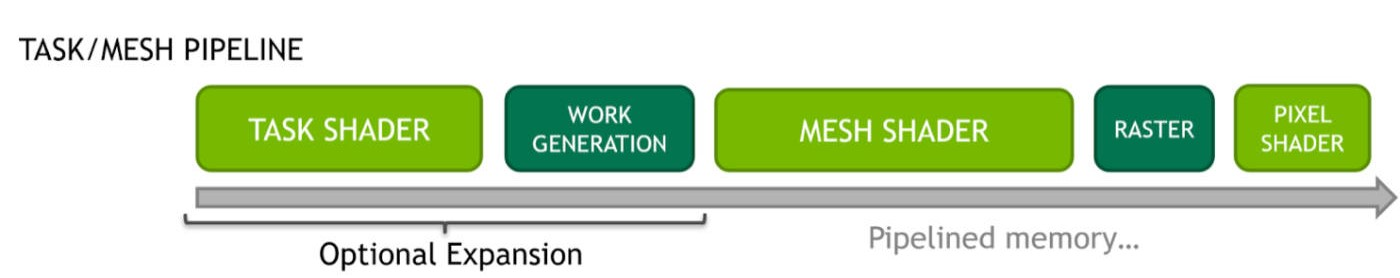
\includegraphics[scale=0.43]{Bilder/Mesh_shading_pipeline.jpg}
  \caption[Mesh Shading Pipeline]{\textbf{Mesh Shading Pipeline} Abbildung der Mesh Shading Pipeline.
  Die Abbildung ist aus dem NVidia Blogpost \cite{Kubisch2018} }
  \label{fig:mesh_shading_pipeline}
\end{figure}

Wie in der Abbildung~\ref{fig:mesh_shading_pipeline} zu sehen ist, durchlaufen die Vertex Daten in der Mesh Shading Pipeline zunächst den Task Shader.
Ähnlich wie bei Compute Shadern (Kap.~\ref{subsec:compute_shader}), werden hier die Anzahl der Workgroups an den Mesh Shader versendet.
Der Mesh Shader arbeitet auf Threads.
Die Ein- und Ausgabe des Mesh Shaders werden vom Entwickler festgelegt.
So können wie beim Compute Shader auch Arbeiten verrichtet werden, die nicht direkt fürs Rendering wichtig sind.
In dieser Arbeit wird der Mesh Shader zum Darstellen des dekomprimierten Dreiecksnetzes genutzt.
Zum Rendern müssen jedoch wieder Fragments ausgegeben werden, die in den unveränderte Rasterisierung und Pixel Shader Stages verarbeitet werden. \cite{Kubisch2018}

\subsubsection*{Mesh Shader}
Da die optionale Task Shader Stage in dieser Arbeit nicht verwendet wird, betrachten wir die Pipeline aus dem Szenario, das die Anzahl an Workgroups des DirectX Dispatch direkt dem Mesh Shader gegeben wird.
Die Nummer an Workgroups beschreibt, wie viele Kerne verwendet werden sollen.
Bei Mesh Shadern bietet es sich an, die Anzahl der Workgroups auf die Anzahl an Meshlets zu setzen.
Jede Workgroup hat außerdem eine Anzahl an Threads.
Die Funktionsweise der Threads wurde bereits im Grundlagenkapitel.~\ref{subsec:compute_shader} erläutert.
Jedem Meshlet wird eine Workgroup zugeteilt.
Jede Workgroup wird wiederum in Threads unterteilt \cite{Kubisch2018}.

\subsection{Meshlets}
\label{subsec:meshlets}
Um die neuartigen Shader für das Rendering zu verwenden, wird empfohlen, das gesamte Mesh in kleinere Subsets, sogenannte Meshlets, zu unterteilen. 
Die traditionelle Grafikpipeline verarbeitet die Daten des Dreiecksnetzes in serieller Manier. 
Dadurch kommt es jedoch zu Bottlenecks.
In der traditionellen Pipeline werden Vertex und Primitiven vor der Vertex Shader Stage zugeschnitten und in kleine Clustern verarbeitet.
Dazu wird der Primitive Distributor vor der Vertex Shader Stage aufgerufen.
Dieser liest die Daten des Index-Buffers und generiert dementsprechend möglichst performant diese Cluster an Daten.
Der Schritt des Primitive Distributor ist jedoch eine fixed-function Stage der Grafikpipeline, wodurch der Entwickler keinen direkten Zugriff hat.
Das hat zur Folge, dass die Cluster nicht auf die Bedürfnisse des Entwicklers und dessen Implementierung angepasst werden können.
Zuzüglich werden die Cluster zu jedem Frame, bzw. vor jedem Aufruf der Pipeline neu generiert.
Dieser Schritt ist redundant, sollte das Dreiecksnetz zur Laufzeit unverändert bleiben \cite{Carvalho2022}, \cite{Kubisch2018}. \newline

Wie beim Compute Shader ist der Input des Mesh Shaders anders als bei der traditionellen Grafikpipeline nicht mehr festgelegt.
Dadurch kann der Entwickler seine eigenen Implementationen zur Generierung von Meshlets verwenden.
Anders als bei der herkömmlichen Grafikpipeline werden Meshlets auf CPU Ebene erstellt.
Dazu werden Vertex Positionen und Indizes benötigt.
Die Anzahl der Vertices und Primitiven muss im Vorfeld festgelegt werden.
Die maximale Größe der Meshlets ist abhängig von der verwendeten GPU.
So wird im NVIDIA Blogpost \textit{Introduction to Turing Mesh Shaders} eine maximale Anzahl an Vertices von 64, und Primitiven von 126 empfohlen.
Die 126 ist bewusst keine Zweierpotenz, da 4 Byte für die Anzahl der Primitiven des Meshlets verwendet werden.
Zur Vermeidung der Anforderung eines zusätzlichen Speicherblocks werden diese 4 Byte Speicher freigelassen \cite{Kubisch2018}. \newline

Arseny Kapoulkine hat verschiedene Meshletgrößen miteinander verglichen.
Er ist zu dem Schluss gekommen, dass 64 Vertices und 84 Primitives am effizientesten sind, insbesondere dann, wenn im Task Shader Culling auf die einzelnen Meshlets angewendet wird.
Des Weiteren ist die Empfehlung des Blogposts nach eigenen Tests zwar ein guter Maßstab, jedoch wird im Durchschnitt viel Speicher des Primitiven Buffers ungenutzt bleiben, da die 126 Primitiven mit 64 Vertices nie erreicht werden \cite{Kapoulkine2023}.

\subsection{Implementierung eines Standard Mesh Shaders}
\label{subsec:standard_meshshaderimpl}
Wie im vorherigen Unterkapitel angekündigt, muss das Dreiecksnetz auf der CPU zu Meshlets geschnitten werden. 
Dazu wurde in dieser Arbeit der Meshoptimizer von Zeux verwendet \cite{Zeux}. 
[Implementierung von Zeux beschreiben]
Die Funktion \glqq meshopt\_buildMeshlets\grqq\ nimmt als Eingabeparameter die maximale Anzahl an Vertices und Primitiven (Kap.\ref{subsec:meshlets}), die Vertex und Index Daten sowie drei leere Buffer.
Der Buffer \textit{meshlet\_indices} wird die neuen Index Daten enthalten, mit denen die Primitiven berechnet werden können.
Der \textit{meshlet\_vertices} Buffer beinhaltet die einzigartigen Vertices des Dreiecksnetzes (Kap~\ref{subsec:local_vertex_buffers}).
Der letzte Buffer wird in dieser Arbeit als \textit{Meshlet Descriptor} bezeichnet.
Der Einfachheit und Übersichtlichkeit halber wird er im Code jedoch einfach als \textit{meshlets} implementiert.
Der Meshlet Buffer setzt sich aus folgenden Elementen zusammen \cite{Jensen2023}.
\begin{itemize}
\item Vertex Count: Die Anzahl der Vertices V in dem Meshlet mit dem Index i
\item Primitive Count: Die Anzahl der Primitives P in dem Meshlet mit dem Index i
\item Vertex Offset: Die Menge an Schritten im Vertex-Buffer, um an die Vertices des i-ten Meshlets zu gelangen
\item Primitive Offset: Die Menge an Schritten im Index-Buffer, um an die Primitives des i-ten Meshlets zu gelangen
\end{itemize} 
Im nächsten Abschnitt wird genauer auf die neuen Buffer eingegangen. \newline

\subsubsection*{Vertex Index}
Um auf einen Vertex zuzugreifen, wird der Buffer meshlet\_vertices benötigt.
Er beinhaltet Ganzzahlen ohne Vorzeichen, die auf einen bestimmten Vertex eines Meshlets zeigen.
Im Codeabschnitt~\ref{lst:shadercode} wir die Variable \textit{vertexIndex} mittels der \textit{GetVertexIndex} Methode gesetzt.
In der Methode wird der lokale Vertex Index mittels
\begin{equation*}
\text{localVertex} = \text{VertexOffset} + \text{localIndex}
\end{equation*}
bestimmt. \newline
Mithilfe des \textit{localIndex} kann nun der Vertex Index aus dem \textit{meshlet\_vertices} Buffer gelesen werden.
Abschließend wird der Vertex mithilfe des Vertex Index aus dem Buffer mit den Vertex-Ressourcen ausgelesen.
Was hierbei festgestellt werden kann, ist, dass eine doppelte Indexierung notwendig ist und somit Informationen aus zwei Buffer ausgelesen werden müssen, um einen Vertex zu lesen.
In einem späteren Abschnitt wird dieses Problem mithilfe von Duplizierung der Vertices gelöst.

\subsubsection*{Primitive Index}
Der Buffer \textit{meshlet\_indices} ist für die Primitiven der Meshlets zuständig.
Ein herkömmlicher Index-Buffer enthält Ganzzahlen ohne Vorzeichen zwischen 0 - \textit{VertexCount - 1}.
Die hier jedoch eine Indexierung auf Meshlet Ebene vorliegt, müssen diese Werte bei gleicher Buffergröße angepasst werden.
Die Werte reichen nun anstelle von 0 - \textit{VertexCount}, von 0 - \textit{MaxPrimitiveCount} - 1.
Das bedeutet, wenn Meshlets mit einer Vertex Anzahl von 64 und Primitiven Anzahl von 128 generiert werden, befinden sich in \textit{meshlet\_indices} lediglich Werte zwischen 0 - 127.
Um den aktuellen Index eines Meshlets zu erhalten, muss ähnlich wie bei den Vertices der lokale Index berechnet werden.
Dazu wird die Formel:
\begin{equation*}
\mathrm{localIndex} = \mathrm{PrimitiveOffset} + (\mathrm{localIndex} \cdot \mathrm{indicesPerTriangle})
\end{equation*}
verwendet.
Da die Ausgabe einen 3-dimensionalen Vektor für die Primitiven erwartet, ist die Variable indicesPerTriangle = 3.
Nun müssen nur noch die drei Indizes des aktuellen Meshlet Index aus dem Buffer gelesen und gesetzt werden.
\newline
Auffällig ist, dass die obere Schranke der Werte, die die Indizes enthalten, bedeutend geringer ist gegenüber eines herkömmlichen Index-Buffers.
Der benötigte Speicher eines einzelnen Indizes wird dadurch drastisch reduziert.
Für einen Index wurden ursprünglich 4-Byte Speicher benötigt.
Für die \textit{meshlet\_indices} werden in dem Fall von \textit{\^{V}} = 128 und \textit{\^{I}} = 256 höchstens 8 Bit für die Repräsentation eines Index benötigt.
Diese Auffälligkeit kann sich zunutze gemacht werden, indem eine Primitive bzw. drei Indizes in ein 4-Byte Integer verpackt werden.
Dadurch kann 66 \% des Speicherbedarfs für den Index-Buffer gespart werden.

Mit den Informationen der originalen Vertex Daten und der drei neu generierten Buffer \textit{meshlet\_indices}, \textit{meshlet\_vertices} und \textit{meshlets}, kann nun der Mesh Shader gefüttert werden.
Zunächst müssen die während des Build-Vorgangs kompilierten Shader gelesen werden.
Diese enthalten Informationen zum Layout der Root Signature, die daraufhin per API-Call erstellt wird.
Bevor die Meshlet Daten an den Mesh Shader übergeben werden können, müssen diese in einen GPU-Buffer und somit in den GPU-RAM geschrieben werden.
Wenn alles erledigt ist, können in der Commandlist der Constant Buffer und die benötigten Meshletdaten über die DirectX12 API-Calls SetGraphicsRootConstantBuffer und SetGraphicsRootShaderRessourceView gesetzt werden.

\subsection{Mesh Shader Implementation}
\label{subsec:mesh_shader_impl}
Im Codeabschnitt~\ref{lst:shadercode} ist ein einfacher Mesh Shader zu sehen.
Im Mesh Shader wird die Root Signature entsprechend den Anforderungen gesetzt.
Minimal wird ein StructuredBuffer für jeden der auf der CPU generierten Meshlet Buffer benötigt.
Um das Endresultat 3-Dimensional wirken zu lassen, wird ein ConstantBuffer verwendet, der die \textit{model}, \textit{modelView} und \textit{modelViewProjection} Matrix beinhaltet.
Zunächst wird das aktuelle Meshlet aus dem \textit{Meshlet Descriptor Buffer} genommen.
Die SV\_GroupID stellt in dieser Implementierung den aktuellen Index der Meshlets dar.
Um den lokalen Index des aktuellen Meshlets zu bekommen, muss die SV\_GroupThreadID verwendet werden.
Die aktuelle GroupID wird in einzelne Threads unterteilt, damit die GPU sich bei der parallelen Verarbeitung nicht in die Queere kommt.
Die Anzahl der Threads wird mittels \textit{[NumThreads(128, 1, 1)]} im Mesh Shader oder, falls vorhanden, im Task Shader festgelegt. \newline

Zu Beginn eines jeden Mesh Shaders muss die Anzahl der auszugebenden Vertices und Primitives mittels \textit{SetMeshOutputCounts} gesetzt werden \cite{Jobalia2019}.
Dafür wurde eine Datenstruktur für den Meshlet Descriptor mit der Struktur wie sie in Kapitel.~\ref{subsec:standard_meshshaderimpl} definiert wurde, erstellt.
Der Meshlet Descriptor mit der aktuellen GroupID wird also aus dem auf CPU-Ebene erstellten Buffer gelesen und die Anzahl der Vertices und Primitiven festgelegt.
Welchen fundamentalen Nutzen der Meshlet Descriptor für einen Mesh Shader hat, kann man hier erkennen.
Die aktuellen Gruppe wird in Threads aufgeteilt, die sich jeweils um einen Vertex und eine Primitive kümmern.
Dazu wird überprüft, ob sich die GroupThreadID noch innerhalb der Grenzen des aktuellen Meshlets befindet.
Sollte dies der Fall sein, liest der Mesh Shader mithilfe des Meshlet Descriptors und der GroupThreadID Vertex und Primitive aus.

\newpage \begin{lstlisting}[language = C++, caption = Main Methode des Mesh Shaders, label=lst:shadercode]
[RootSignature(ROOT_SIG)]
[NumThreads(128, 1, 1)]
[OutputTopology("triangle")]
void main(
    in uint localIndex : SV_GroupThreadID,
    in uint meshletIndex : SV_GroupID,
    out vertices VertexOut verts[64],
    out indices uint3 tris[128]
)
{
  	Meshlet m = Meshlets[meshletIndex];

	SetMeshOutputCounts(m.VertCount, m.PrimCount);

	if (localIndex < m.PrimCount)
	{
  		tris[localIndex] = GetPrimitive(m, localIndex);
	}

	if (drawQuantizedVertices)
	{
  		if (localIndex < m.VertCount)
  		{
    		verts[localIndex] = GetQuantizedVertex(meshletIndex, localIndex);
  		}
	}
	else
	{
  		if (localIndex < m.VertCount)
  		{
    		verts[localIndex] = GetVertex(meshletIndex, localIndex);
  		}
	}
}
\end{lstlisting}

\subsection{Lokale Vertex-Buffer}
\label{subsec:local_vertex_buffers}
Der Mesh Shader im Codeabschnitt.~\ref{lst:shadercode} zeigt eine Implementierung in seiner einfachsten Form.
Der Plan ist jedoch, jedes Meshlet einzeln zu dekodieren, um die dekodierten Meshletdaten zu rendern.
Der originale Vertex und Index-Buffer müssen dafür angepasst werden.
In Kap.~\ref{subsec:standard_meshshaderimpl} wurden bereits die benötigten Buffer erklärt, die der Meshoptimizer generiert.
Vertex und Index-Buffer werden mit diesem anpasst, damit jedes Meshlet über die gewünschte Geometrie und Topologie verfügt. \newline
Um den Punkt der doppelten Indexierung des Vertex-Buffers einzugehen, werden in diesem Abschnitt lokale Vertex-Buffer für jedes Meshlet generiert.
Die duplizierten Vertex Daten werden in Kauf genommen, damit sich während des Renderns ein zusätzlicher Elementzugriff gespart werden kann.
\newline
Das Ziel ist es, die Vertex Daten auf die generierten Meshlets anzupassen, damit die Vertices der Meshlets sequentiell in einem Buffer liegen, wie es in Abb.~\ref{fig:local_vertex_buffer} illustriert ist.
\begin{figure}[htb]
  \centering  
  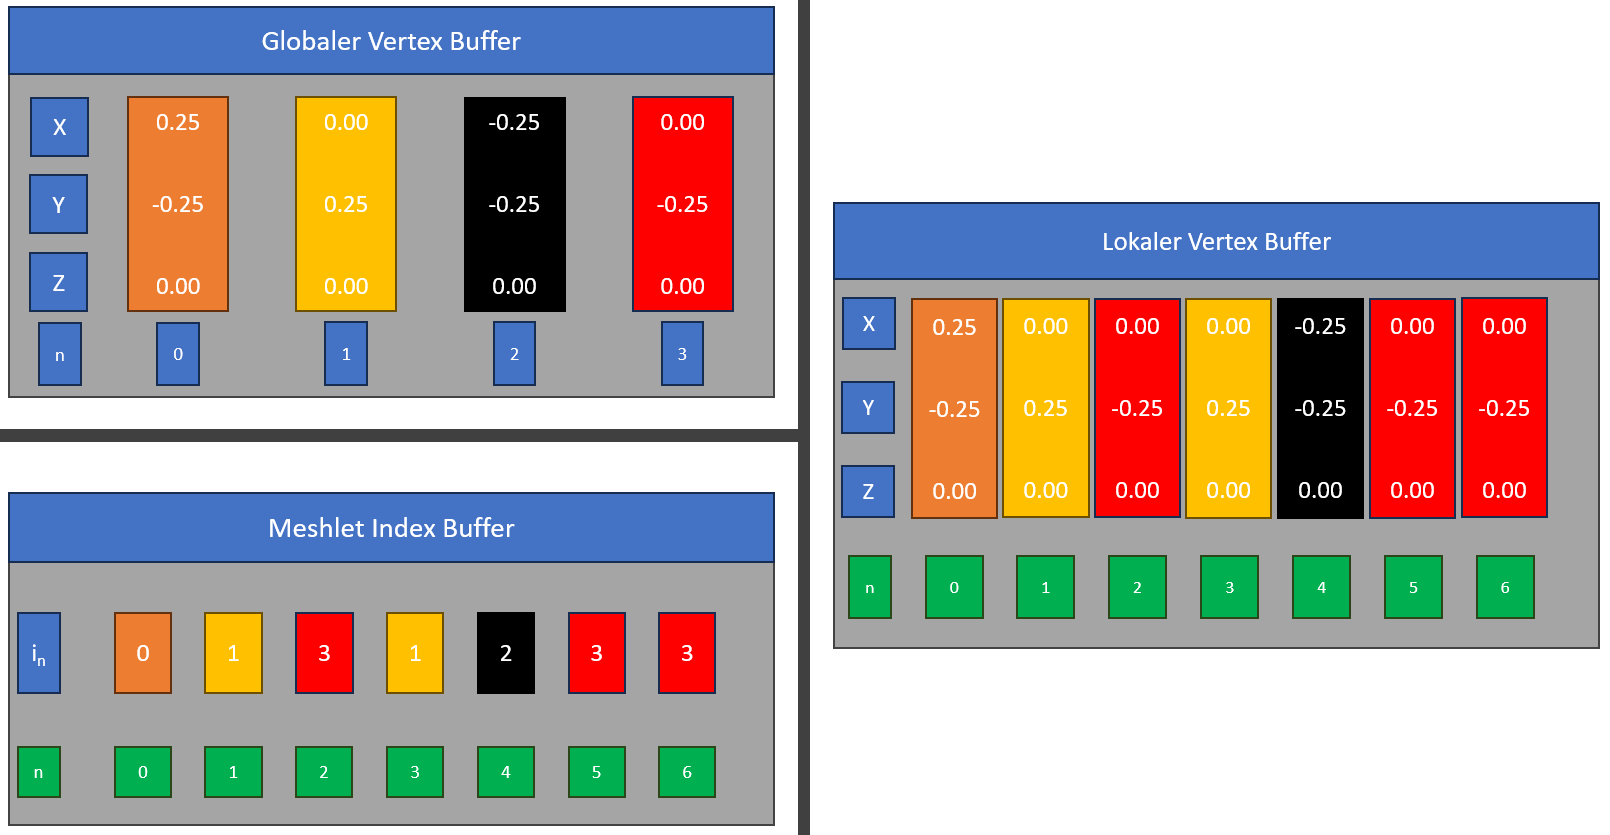
\includegraphics[scale=0.375]{Bilder/local_vertex_buffer.png}
  \caption[Lokaler Vertex-Buffer]{\textbf{Lokaler Vertex-Buffer} Die Abbildung zeigt eine Konstruktion eines Vertex-Buffers der die Vertices aller Meshlets sequentiell beinhaltet.}
  \label{fig:local_vertex_buffer}
\end{figure}

In der Methode GetVertexIndex musste zunächst ein \textit{Unique Vertex Index} berechnet werden, der den Index für den globalen Vertex-Buffer bereitgestellt hat.
Mithilfe des lokalen Vertex-Buffers ist dieser Schritt nicht mehr nötig.
Der korrekte Vertex Index kann nun lediglich mit dem Vertex Offset des Meshlets und der GroupThreadID berechnet werden.
Mit diesem Index ist ein direkter Zugriff auf die Vertex-Ressourcen möglich.
Dadurch befinden sich zwar duplizierte Vertices im Vertex-Buffer, der Buffer mit den \textit{Unique Vertex Indices} wird jedoch nicht mehr benötigt.
Darauf folgt noch, dass der zusätzliche Elementzugriff des wegfallenden Buffers nicht mehr notwendig ist, um zu den jeweiligen Meshlet Vertex zu gelangen.
So besteht jeder einzelne, große Buffer mit allen Elementen sozusagen aus zusammengesetzten, kleinen Meshlet Buffern.